\documentclass{article}
\usepackage{amsmath,amsthm,amssymb}
\usepackage[T1,T2A]{fontenc}
\usepackage[utf8]{inputenc}
\usepackage[english,russian]{babel}
\usepackage{graphicx}%Вставка картинок правильная
\usepackage{float}%"Плавающие" картинки
\usepackage{wrapfig}%Обтекание фигур (таблиц, картинок и прочего)
\begin{document}

	\subsection*{1. Найти функицю, которая на $+ \infty$ растёт как линейная функиция, а на $- \infty$ ведёт себя как константа}
	Путём долгих изысканий, я нашёл следующую функцию:
	$f(x) = \frac{x^3}{x^2 + e^{-x}}$
	\\
	Проверим её на соответсвие заданным условиям:
	\begin{itemize}
		\item 	наклонная асимптота на $+ \infty$:
		\begin{gather*}
			\lim_{x\to + \infty} \frac{f(x)}{x} = \lim_{x\to + \infty} \frac{x^3}{x(x^2 + e^{-x})}=\lim_{x\to + \infty} \frac{x^2}{x^2 + e^{-x}}=\lim_{x\to + \infty} \frac{1}{1 + \frac {e^{-x}}{x^2}}=\frac{1}{\lim_{x\to + \infty} \left( 1 + \frac {e^{-x}}{x^2}\right) } =\nonumber \\ =\frac{1}{\lim_{x\to + \infty} \left( 1 + \frac {e^{-x}}{x^2}\right) } = \frac{1}{1 + \lim_{x\to + \infty} \left(\frac {1}{x^2 \cdot e^{x}}\right) } = \frac{1}{1 + \frac{1}{\infty} } = \frac{1}{1 + 0} = 1 \in R
			\end{gather*}
				\item 	поведение константы на $- \infty$:
			\begin{gather*}
			\lim_{x\to + \infty} \frac{f(x)}{x} = \lim_{x\to - \infty} \frac{x^3}{x(x^2 + e^{-x})}=\lim_{x\to - \infty} \frac{x^2}{x^2 + e^{-x}}=\lim_{x\to - \infty} \frac{1}{1 + \frac {e^{-x}}{x^2}}=\frac{1}{\lim_{x\to - \infty} \left( 1 + \frac {e^{-x}}{x^2}\right) } =\nonumber \\ =\frac{1}{\lim_{x\to - \infty} \left( 1 + \frac {e^{-x}}{x^2}\right) } = \frac{1}{1 + \lim_{x\to - \infty}\left( \frac {e^{-x}}{x^2}\right) } = \frac{1}{1 + \infty } = \frac{1}{+\infty} = 0 \in R
			\end{gather*}
	\end{itemize}
	Таким образом, у заданной функции $f(x) = \frac{x^3}{x^2 + e^{-x}}$ есть две асимптоты: на $+\infty$ это прямая вида $y = 1 \cdot x + b$, на $-\infty$ это горизонтальная прямая $y = 0$.
	\begin{figure}[h]
		\centering
		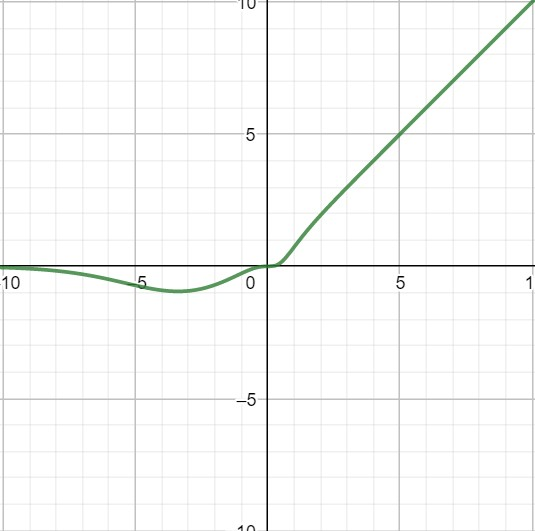
\includegraphics[width=0.5\linewidth]{plot_task_1.jpg}
		
		\caption{Диаграмма моментов на участке выбора момента прокатки}
		
		\label{fig:mpr}
		
	\end{figure}
\end{document}